%%%%%%%%%%%%%%%%%%%%%%%%%%%%%%%%%%%%%%%%%%%%%%%%%%%%%%%%%%%%%%%%%%%%%%%%%
% This file is part of the LaTeX sources of the OMDoc 1.6 specification
% Copyright (c) 2006 Michael Kohlhase
% This work is licensed by the Creative Commons Share-Alike license
% see http://creativecommons.org/licenses/by-sa/2.5/ for details
% The source original is at https://github.com/KWARC/OMDoc/doc/spec 
%%%%%%%%%%%%%%%%%%%%%%%%%%%%%%%%%%%%%%%%%%%%%%%%%%%%%%%%%%%%%%%%%%%%%%%%%

\begin{omgroup}[short=Mathematical Statements,id=statements]
{Mathematical Statements (Module {\STmodule{spec}})}

  In this chapter we will look at the \omdoc infrastructure to mark up the
  {\emph{functional structure}} of {\twintoo{mathematical}{statement}s} and their
  interaction with a broader mathematical context.
  
\begin{omgroup}[id=statements-constitutive]{Types of Statements in Mathematics}
\begin{module}[id=statementtypes]

  In the last chapter we introduced mathematical statements as special text fragments that
  state properties of the mathematical objects under discussion and categorized them as
  definitions, theorems, proofs,\ldots. A set of statements about a related set of objects
  make up the context that is needed to understand other statements.  For instance, to
  understand a particular theorem about finite groups, we need to understand the
  definition of a group, its properties, and some basic facts about finite groups
  first. Thus statements interact with context in two ways: the context is built up from
  (clusters of) statements, and statements only make sense with reference to a context. Of
  course this dual interaction of statements with {\emph{context}}\footnote{In linguistics
    and the philosophy of language this phenomenon is studied under the heading of
    ``{\indexalt{discourse theories}{discourse theory}}'', see e.g.~\cite{KamRey:fdtl93}
    for a start and references.}  applies to any text and to communication in general. In
  mathematics, where the problem is aggravated by the load of notation and the need for
  precision for the communicated concepts and objects, contexts are often discussed under
  the label of \twinalt{mathematical theories}{mathematical}{theory}. We will distinguish
  two classes of statements with respect to their interaction with theories: We view
  {\indextoo{axiom}s} and {\indextoo{definition}s} as {\emph{constitutive}} for a given
  theory, since changing this information will yield a different theory (with different
  mathematical properties, see the discussion in {\extref{book}{meta-math}}).  Other
  mathematical statements like {\indextoo{theorem}s} or the {\indextoo{proof}s} that
  support them are not constitutive, since they only illustrate the mathematical objects
  in the theory by explicitly stating the properties that are implicitly determined by the
  constitutive statements.
  
\begin{omtext}
To support this notion of context \omdoc supports an infrastructure for theories using
special \element{theory} elements, which we will introduce in {\sref{theories-contexts}} and
extend in {\sref{complex-theories}}.
\twinalt{Theory-constitutive}{theory-constitutive}{element} elements must be contained as
children in a \element{theory} element; we will discuss them in
{\sref{definitions}}, non-constitutive statements will be defined in
{\sref{assertion}}. They are allowed to occur outside a \element{theory} element in
\omdoc documents (e.g. as top-level elements), however, if they do they must reference a
theory, \inlinedef{which we will call their \defii{home}{theory}} in a special
\attribute{theory}{statement} attribute. This situates them into the context provided by
this theory and gives them access to all its knowledge. The home theory of
theory-constitutive statements is given by the theory they are contained in.
\end{omtext}

The division of statements into constitutive and non-constitutive ones and the
encapsulation of constitutive elements in \element{theory} elements add a certain
measure of safety to the knowledge management aspect of \omdoc.  Since {\xml} elements
cannot straddle document borders, all constitutive parts of a theory must be contained in
a single document; no constitutive elements can be added later (by other authors), since
this would change the meaning of the theory on which other documents may depend on.
  
Before we introduce the \omdoc elements for theory-constitutive statements, let us
fortify our intuition by considering some mathematical examples.  {\emph{Axioms}} are
assertions about (sets of) mathematical objects and concepts that are assumed to be
true. There are many forms of axiomatic restrictions of meaning in mathematics. Maybe the
best-known are the five Peano Axioms for natural numbers.

\begin{myfig}{peano}{The Peano Axioms}
  \fbox{\begin{minipage}{11cm}
 \begin{enumerate}
 \item 0 is a natural number.
 \item The successor $s(n)$ of a natural number $n$ is a natural number.
 \item 0 is not a successor of any natural number.
 \item The successor function is one-one (i.e. injective).
 \item The set $\NN$ of natural numbers contains only elements that can be
   constructed by axioms 1. and 2.
 \end{enumerate}
 \end{minipage}}
\end{myfig}

\begin{omtext}
The {\twintoo{Peano}{axioms}} in {\myfigref{peano}} (implicitly) introduce three
{\indextoo{symbol}s}: the number 0, the successor function $s$, and the set $\NN$ of
natural numbers. The five axioms in {\myfigref{peano}} jointly constrain their meaning
such that conforming structures exist (the natural numbers we all know and love) any two
structures that interpret 0, $s$, and $\NN$ and satisfy these axioms must be isomorphic.
This is an ideal situation --- the axioms are neither too lax (they allow too many
mathematical structures) or too strict (there are no mathematical structures) --- which is
difficult to obtain. The latter condition (\inlinedef{\defi{inconsistent} theories}) is
especially unsatisfactory, since any statement is a theorem in such theories. As
consistency can easily be lost by adding axioms, mathematicians try to keep
{\twintoo{axiom}{system}s} minimal and only add axioms that are safe.
\end{omtext}

\begin{omtext}
  Sometimes, we can determine that an axiom does not destroy {\indextoo{consistency}} of a
  theory $\cT$ by just looking at its form: for instance, axioms of the form $s=\bA$,
  where $s$ is a symbol that does not occur in $\cT$ and $\bA$ is a formula containing
  only symbols from $\cT$ will introduce no constraints on the meaning of
  $\cT$-symbols. The axiom $s=\bA$ only constrains the meaning of the
  {\twintoo{new}{symbol}} to be a unique object: the one denoted by $\bA$. \inlinedef{We
    speak of a \defii{conservative}{extension} in this case}. So, if $\cT$ was a
  consistent theory, the extension of $\cT$ with the symbol $s$ and the axiom $s=\bA$ must
  be one too. Thus axioms that result in {\twintoo{conservative}{extension}s} can be added
  safely --- i.e. without endangering consistency --- to theories.
\end{omtext}

\begin{definition}[display=flow,id=conservative-extension.def]
  Generally an axiom $\cA$ that results in a {\twintoo{conservative}{extension}} is called
  a \defi{definition} and any new symbol it introduces a \defi{definiendum} (usually
  marked e.g. in boldface font in mathematical texts), and we call \defi{definiens} the
  material in the definition that determines the meaning of the definiendum.
\end{definition}
\end{module}
\end{omgroup}

\begin{omgroup}[id=constitutive-statements]{Theory-Constitutive Statements in OMDoc}
\begin{module}[id=constitutive-statements]

  The \omdoc format provides an infrastructure for four kinds of theory-constitutive
  statements: symbol declarations, type declarations, (proper) axioms, and definitions. We
  will take a look at all of them now.

\begin{presonly}
  \begin{myfig}{constitutive-theory}{Theory-Constitutive Elements in \omdoc}
    \begin{scriptsize}
      \begin{tabular}{|>{\snippet}l|>{\tt}l|>{\tt}p{3.6truecm}|c|>{\tt}p{3.2truecm}|}\hline
        {\rm Element}& \multicolumn{2}{l|}{Attributes\hspace*{2.25cm}} & M & Content  \\\hline
                     & {\rm Required}  & {\rm Optional}                & C &          \\\hline\hline
          symbol     & name      & xml:id, role, scope, style, class   & +  & type*\\\hline
          type       &           & xml:id, system, style, class        & -- & h:p*,\llquote{mobj}      \\\hline
          axiom      & name      & xml:id, for, type, style, class     & +  & h:*,FMP*   \\\hline
          definition & for & xml:id, type, style, class                & +  & h:p*, \llquote{mobj})?  \\\hline
 \multicolumn{5}{|l|}{where \llquote{mobj} is {\tt{(\mobjabbr)}}}\\\hline
\end{tabular}
\end{scriptsize}
\end{myfig}
\end{presonly}

\begin{omgroup}[id=symbol-dec]{Symbol Declarations}

  The {\element{symbol}} element declares a symbol for a
  {\twintoo{mathematical}{concept}}, such as 1 for the natural number ``one'', $+$ for
  addition, $=$ for equality, or {\snippetin{group}} for the property of being a
  group. Note that we not only use the \element{symbol} element for mathematical objects
  that are usually written with mathematical symbols, but also for any concept or object
  that has a definition or is restricted in its meaning by axioms.
  
We will refer to the mathematical object declared by a \element{symbol} element as a
``{\indextoo{symbol}}'', iff it is usually communicated by specialized notation in
mathematical practice, and as a ``{\indextoo{concept}}'' otherwise.  The name ``symbol''
of the \element{symbol} element in \omdoc is in accordance with usage in the
philosophical literature (see e.g.~\cite{NewSim:cseisas81}): A {\defemph{symbol}} is a
{\emph{{\twinalt{mental}{physical}{representation}} or
    {\twinalt{physical}{mental}{representation}}}} representation of a concept.  In
particular, a symbol may, but need not be representable by a (set of) {\indextoo{glyph}s}
(symbolic notation).  The definiendum objects in {\myfigref{math-def}} would be considered
as ``symbols'' while the concept of a ``group'' in mathematics would be called a
``concept''.
  
\begin{definition}[id=symbol.def]
  The {\eldef{symbol}} element has a required attribute \attribute{name}{symbol} whose
  value uniquely identifies it in a theory.  Since the value of this attribute will be
  used as an {\openmath} symbol name, it must be an {\xml} name\footnote{This limits the
    characters allowed in a name to a subset of the characters in Unicode 2.0; e.g. the
    colon $\colon$ is not allowed. Note that this is not a problem, since the name is just
    used for identification, and does not necessarily specify how a symbol is presented to
    the human reader. For that, \omdoc provides the notation definition infrastructure
    presented in {\sref{pres}}.} as defined in {\xml} 1.1~\cite{xml1.1:04}. The optional
  attribute \attribute{scope}{symbol} takes the values \attribute{global}{scope}{symbol}
  and \attval{local}{scope}{symbol}, and allows a simple specification of visibility
  conditions: if the \attribute{scope}{symbol} attribute of a \element{symbol} has
  value \attval{local}{scope}{symbol}, then it is not \twinalt{exported}{export}{symbol}
  outside the theory; The {\oldattribute{scope}{symbol}{1.2}} attribute is deprecated, a
  formalization using the \attribute{hiding}{imports} attribute on the
  \element{imports} element should be used instead.  Finally, the optional attribute
  \attribute{role}{symbol} that can take the values\footnote{The first six values come
    from the {\openmath}2 standard. They are specified in content dictionaries; therefore
    \omdoc also supplies them.}
\begin{description}
\item[\attval{binder}{role}{symbol}] The symbol may appear as a binding symbol of an
  {\twintoo{binding}{object}}, i.e. as the first child of an \element[ns-elt=om]{OMBIND}
  object, or as the first child of an \element[ns-elt=m]{apply} element that has an
  \element[ns-elt=m]{bvar} as a second child.
\item[\attval{attribution}{role}{symbol}] The symbol may be used as key in an
  {\openmath} \element[ns-elt=om]{OMATTR} element, i.e. as the first element of a
  key-value pair, or in an equivalent context (for example to refer to the value of an
  attribution).  This form of attribution may be ignored by an application, so should be
  used for information which does not change the meaning of the attributed {\openmath}
  object.
\item[\attval{semantic-attribution}{role}{symbol}] This is the same as
  {\attvalveryshort{attribution}} except that it modifies the meaning of the attributed
  {\openmath} object and thus cannot be ignored by an application.
\item[\attval{error}{role}{symbol}] The symbol can only appear as the first child of an
  {\openmath} error object.
\item[\attval{application}{role}{symbol}] The symbol may appear as the first child of an
  application object.
\item[\attval{constant}{role}{symbol}] The symbol cannot be used to construct a compound
  object.
\item[\attval{type}{role}{symbol}] The symbol denotes a sets that is used in a type
  systems to annotate mathematical objects.
\item[\attval{sort}{role}{symbol}] The symbol is used for a set that are inductively
  built up from constructor symbols; see {\sref{adt}}.
\end{description}
If the \attribute{role}{symbol} is not present, the value
\attval{object}{role}{symbol} is assumed.

The children of the \element{symbol} element consist of a
{\twintoo{multi-system}{group}} of \element{type} elements (see {\sref{type-axioms}} for
a discussion). For this group the order does not matter.  In {\mylstref{symbol}} we have a
symbol declaration for the concept of a {\indextoo{monoid}}.  Keywords or simple phrases
that describes the symbol in mathematical vernacular can be added in the
\element{metadata} child of \element{symbol} as \element[ns-elt=dc]{subject} and
{\element[ns-elt=dc]{description}s}; the latter have the same content model as the
\element{h:p} elements, see the discussion in {\sref{mtext}}). If the document
containing their parent \element{symbol} element were stored in a data base system, it
could be looked up via these metadata. As a consequence the symbol
\attribute{name}{symbol} need only be used for identification. In particular, it need
not be mnemonic, though it can be, and it need not be language-dependent, since this can
be done by suitable \element[ns-elt=dc]{subject} elements.
\end{definition}

\begin{lstlisting}[label=lst:symbol,mathescape,
  caption={An \omdoc \element{symbol} Declaration},
  index={symbol,type}]
<symbol name="monoid">
  <metadata>
    <dc:subject xml:lang="en">monoid</dc:subject>
    <dc:subject xml:lang="de">Monoid</dc:subject>
    <dc:subject xml:lang="it">monoide</dc:subject>
  </metadata>
  <type system="simply-typed">$set[any]\rightarrow(any\rightarrow any \rightarrow any)\rightarrow any\rightarrow bool$</type>
  <type system="props">
    <OMS cd="arities" name="ternary-relation"/>
  </type>
</symbol>
\end{lstlisting}
\end{omgroup}

\begin{omgroup}[id=axioms]{Axioms}
  
  The relation between the components of a monoid would typically be specified by a set of
  axioms (e.g. stating that the base set is closed under the operation).  For this purpose
  \omdoc uses the \element{axiom} element:

\begin{definition}[id=axiom.def]
  The {\eldef{axiom}} element contains mathematical vernacular as a sequence of
  \element[ns-elt=h]{p} elements a \element{FMP} that expresses this as a logical
  formula.  \element{axiom} elements may have a \attribute{generated-from}{axiom}
  attribute, which points to another \omdoc element (e.g. an \element{adt}, see
  {\sref{adt}}) which subsumes it, since it is a more succinct representation of the same
  mathematical content. Finally the \element{axiom} element has an optional
  \attribute{for}{axiom} attribute to specify salient semantic objects it uses as a
  {\indextoo{whitespace-separated list}} of {\indextoo{URI}} references to symbols
  declared in the same theory, see {\mylstref{axiom}} for an example. Finally, the
  \element{axiom} element can have an \attribute{type}{axiom} attribute, whose values
  we leave unspecified for the moment.
\end{definition}

\begin{lstlisting}[label=lst:axiom,mathescape,
  caption={An \omdoc \element{axiom}},index={axiom}]
<axiom xml:id="mon.ax" for="monoid">
  <h:p>If $\psom{(M,*)}$ is a semigroup with unit $\psom{e}$, then $\psom{(M,*,e)}$ is a monoid.</h:p>
</axiom>
\end{lstlisting}
\end{omgroup}

\begin{omgroup}[id=type-axioms]{Type Declarations}

\begin{omtext}
  {\indexalt{Types}{type}} (also called {\indextoo{sort}s} in some contexts) are
  representations of certain simple sets that are treated specially in (human or
  mechanical) {\twintoo{reasoning}{process}es}. \inlinedef{A \defii{type}{declaration}
    $e\colon t$ makes the information that a symbol or expression $e$ is in a set
    represented by a type $t$ available to a specified mathematical process}.  For
  instance, we might know that $7$ is a natural number, or that expressions of the form
  $\sum_{i=1}^n a_ix^{i}$ are polynomials, if the $a_i$ are real numbers, and exploit this
  information in mathematical processes like proving, pattern matching, or while choosing
  intuitive notations.  \inlinedef{If a type is declared for an expression that is not a
    symbol, we will speak of a \defii{term}{declaration}}.
\end{omtext}

\begin{definition} [id=type.def]
  \omdoc uses the {\eldef{type}} element for type declarations. The optional attribute
  \attribute{system}{type} contains a {\indextoo{URI}} reference that identifies the
  {\twintoo{type}{system}} which interprets the content. There may be various sources of
  the set membership information conveyed by a type declaration, to justify it this source
  may be specified in the optional \attribute{just-by}{type} attribute. The value of
  this attribute is a {\indextoo{URI}} reference that points to an \element{assertion}
  or \element{axiom} element that asserts $\allcdot{x_1,\ldots,x_n}{e\in t}$ for a type
  declaration $e\colon t$ with variables $x_1,\ldots,x_n$.  If the
  \attribute{just-by}{type} attribute is not present, then the type declaration is
  considered to be generated by an {\twintoo{implicit}{axiom}}, which is considered
  {\indextoo{theory-constitutive}}\footnote{It is considered good practice to make the
    axiom explicit in formal contexts, as this allows an extended automation of the
    knowledge management process.}.
  
  The \element{type} element contains one or two mathematical objects. In the first
  case, it represents a type declaration for a symbol (we call this a
  \defii{symbol}{declaration}), which can be specified in the optional
  \attribute{for}{type} attribute or by embedding the \element{type} element into the
  respective \element{symbol} element.  A \element{type} element with two mathematical
  objects represents a {\twintoo{term}{declaration}} $e\colon t$, where the first object
  represents the expression $e$ and the second one the type $t$ (see
  {\mylstref{term-declaration}} for an example). There the type declaration of
  {\snippet{monoid}} characterizes a monoid as a three-place predicate (taking as
  arguments the base set, the operation, and a neutral element).
\end{definition}    

\begin{omtext}
  As reasoning processes vary, information pertaining to multiple
  {\twintoo{type}{system}s} may be associated with a single symbol and there can be more
  than one \element{type} declaration per expression and {\twintoo{type}{system}}, this
  just means that the object has more than one type in the respective type system (not all
  type systems admit {\twintoo{principal}{type}s}).
\end{omtext}
\end{omgroup}

\begin{omgroup}[id=definitions]{Definitions}

Definitions are a special class {\indextoo{axioms}} that completely fix the meaning of
symbols. 

\begin{definition}[id=definition.def]
  Therefore {\eldef{definition}} elements that represent definitions carry the required
  \attribute{for}{definition} attribute, which contain a whitespace-separated list of
  names of symbols in the same theory.  We call these symbols
  \adefii{defined}{defined}{symbol} and \adefii{primitive}{primitive}{symbol}
  otherwise. A \element{definition} contains mathematical vernacular as a sequen ce of
  \element[ns-elt=h]{p} elements to describe the meaning of the defined symbols.

  A \element{definition} element contains a mathematical object that can be substituted
  for the symbol specified in the \attribute{for}{definition} attribute of the
  definition. The \attribute{type}{definition} is fixed to
  \attval{simple}{type}{definition}\ednote{maybe better leave it out}.  {\Mylstref{one}}
  gives an example of a simple definition of the number one from the successor function
  and zero. \omdoc treats the \attribute{type}{definition} attribute as an optional
  attribute. If it is not given explicitly, it defaults to
  \attval{simple}{type}{definition}.
\end{definition}

\begin{lstlisting}[label=lst:one,
  caption={A Simple \omdoc \element{definition}.},
  index={definition}]
<symbol name="one"/>
<definition xml:id="one.def" for="one" type="simple">
 <h:p><OMS cd="nat" name="one"/> is the successor of <om:OMS cd="nat" name="zero"/>.</h:p>
 <om:OMA>
   <om:OMS cd="int" name="suc"/>
   <om:OMS cd="nat" name="zero"/>
 </om:OMA>
</definition>
\end{lstlisting}
\end{omgroup}
\end{module}
\end{omgroup}

\begin{omgroup}[id=assertion]{The Unassuming Rest}
\begin{module}[id=non-constitutive-statements]

The bulk of mathematical knowledge is in form of statements that are not
theory-constitutive: statements of properties of mathematical objects that are entailed by
the theory-constitutive ones. As such, these statements are logically redundant, they do
not add new information about the mathematical objects, but they do make their properties
explicit. In practice, the entailment is confirmed e.g.  by exhibiting a proof of the
assertion; we will introduce the infrastructure for proofs in {\sref{proofs}}.

\begin{presonly}
\begin{myfig}{qttheory}{Assertions, Examples, and Alternatives in \omdoc}
\begin{scriptsize}
\begin{tabular}{|>{\tt}l|>{\tt}p{2truecm}|>{\tt}p{3truecm}|c|>{\tt}p{2.8truecm}|}\hline
{\rm Element}& \multicolumn{2}{l|}{Attributes\hspace*{2.25cm}} & M & Content  \\\hline
             & {\rm Required}  & {\rm Optional}                & D &           \\\hline\hline
 assertion   &      & xml:id, type, theory, class, style, status, just-by  & +
             & h:p*, FMP*      \\\hline
 type        & system  & xml:id, for, just-by, theory, class, style      
                                     & -- & h:p*, \llquote{mobj},\llquote{mobj}\\\hline
 example     & for & xml:id, type, assertion, theory, class, style 
                                     & +  & h:p* | \llquote{mobj}*  \\\hline
 alternative & for, theory, entailed-by, entails, entailed-by-thm, entails-thm  
                & xml:id, type, theory, class, style & +  
                & h:p*, (FMP* | requation* | \llquote{mobj})  \\\hline
 \multicolumn{5}{|l|}{where \llquote{mobj} is {\tt{(\mobjabbr)}}}\\\hline
\end{tabular}
\end{scriptsize}
\end{myfig}
\end{presonly}

\begin{omgroup}[id=assertions]{Assertions}

\begin{definition}[id=assertion.def]
  \omdoc uses the {\eldef{assertion}} element for all statements (proven or not) about
  mathematical objects (see {\mylstref{assertion}}) that are not axiomatic
  (i.e. constitutive for the meaning of the concepts or symbols involved).  Traditional
  mathematical documents discern various kinds of these: {\indextoo{theorem}s},
  \indexalt{lemmata}{lemma}, \indexalt{corollaries}{corollary}, {\indextoo{conjecture}s},
  {\indextoo{problem}s}, etc.

These all have the same structure (formally, a closed logical formula). Their differences
are largely pragmatic (e.g. theorems are normally more important in some theory than lemmata)
or proof-theoretic (conjectures become theorems once there is a proof).  Therefore, we
represent them in the general \element{assertion} element and leave the type distinction
to a \attribute{type}{assertion} attribute, which can have the values in
{\myfigref{assertion-types}}.
\end{definition}

\begin{myfig}{assertion-types}{Types of Mathematical Assertions}
  \begin{tabular}{|l|l|}\hline
    Value & Explanation \\\hline\hline
    \attval{theorem}{type}{assertion}, \attval{proposition}{type}{assertion} 
    & an important assertion with a proof\\\hline 
    \multicolumn{2}{|p{11.3cm}|}{ Note that the meaning of the
      \attribute{type}{assertion} (in this case the existence of a proof) is not
      enforced by \omdoc applications. It can be appropriate to give an assertion
      the \attribute{type}{assertion} \attribute{theorem}{type}{assertion}, if the
      author knows of a proof (e.g. in the literature), but has not formalized it in
      \omdoc yet.}\\\hline\hline
    \attval{lemma}{type}{assertion} & a less important assertion with a proof\\\hline
    \multicolumn{2}{|p{11.3cm}|}{ The difference of importance specified in this
      \attribute{type}{assertion} is even softer than the other ones, since e.g. reusing
      a mathematical paper as a chapter in a larger monograph, may make it necessary to
      downgrade a theorem (e.g.  the main theorem of the paper) and give it the status of
      a lemma in the overall work.}\\\hline\hline
    \attval{corollary}{type}{assertion} & a simple consequence\\\hline
    \multicolumn{2}{|p{11.3cm}|}{ An assertion is
      sometimes marked as a corollary to some other statement, if the proof is
      considered simple. This is often the case for important theorems that are simple
      to get from technical lemmata.}\\\hline\hline
    \attval{postulate}{type}{assertion}, \attval{conjecture}{type}{assertion}
    & an assertion without proof or counter-exam\-ple\\\hline
    \multicolumn{2}{|p{11.3cm}|}{ Conjectures are assertions, whose
      semantic value is not yet decided, but which the author considers likely to be
      true. In particular, there is no proof or counter-example (see
      {\sref{examples}}).}\\\hline\hline
    \attval{false-conjecture}{type}{assertion} 
    & an assertion with a counter-example\\\hline
    \multicolumn{2}{|p{11.3cm}|}{ A conjecture that has proven to be false,
      i.e. it has a counter-example. Such assertions are often kept for illustration and
      historical purposes.}\\\hline\hline
    \attval{obligation}{type}{assertion}, \attval{assumption}{type}{assertion} 
    & an assertion on which the proof of another depends\\\hline
    \multicolumn{2}{|p{11.3cm}|}{ These kinds of assertions
      are convenient during the exploration of a mathematical theory. They can be used
      and proven later (or assumed as an axiom).}\\\hline\hline
    \attval{formula}{type}{assertion} & if everything else fails\\\hline
    \multicolumn{2}{|p{11.3cm}|}{ This type is the catch-all if none of the others
      applies.}\\\hline 
  \end{tabular}
\end{myfig}

\begin{definition}[id=assertion.def]
  The \element{assertion} element also takes an optional
  \attribute[ns-attr=xml]{id}{assertion} element that allows to reference it in a
  document, an optional \attribute{theory}{assertion} attribute to specify the
  {\indextoo{theory}} that provides the {\indextoo{context}} for this assertion, and an
  optional attribute \attribute{generated-from}{assertion}, that points to a higher
  syntactic construct that generates these assertions, e.g. an abstract data type
  declaration given by an \element{adt} element (see {\sref{adt}}).
\end{definition}  

\begin{lstlisting}[label=lst:assertion,mathescape,
  caption={An \omdoc Assertion About Semigroups},
  index={assertion}]
<assertion xml:id="ida.c6s1p4.l1" type="lemma">
  <h:p> A semigroup has at most one unit.</h:p>
  <FMP>$\allcdot{S}{sgrp(S)\rightarrow\allcdot{x,y}{unit(x,S)\wedge unit(y,S)\rightarrow x=y}}$</FMP>
</assertion>
\end{lstlisting}

To specify its proof-theoretic status of an assertion \element{assertion} carries the
two optional attributes \attribute{status}{assertion} and
\attribute{just-by}{assertion}. The first contains a keyword for the status and the
second a whitespace-separated list of {\twintoo{URI}{reference}s} to \omdoc elements
that justify this status of the assertion. For the specification of the status we adapt an
ontology for deductive states of assertion from~\cite{SutZimSch:tdefatpt04} (see
{\myfigref{proof-status}}). Note that the states in {\myfigref{proof-status}} are not
mutually exclusive, but have the inclusions depicted in
{\myfigref{proof-status-taxonomy}}.

\begin{myfig}{proof-status}{Proof Status for Assertions in a Theory $\cT$}
\def\mc#1{\multicolumn{2}{|p{10.7cm}|}{\emph{#1}}}
\begin{footnotesize}
\begin{tabular}{|l|l|}\hline
  \attribute{status}{assertion} & \attribute{just-by}{assertion} points to\\\hline\hline
  \attval{tautology}{status}{assertion} &
  Proof of $\cF$\\
  \mc{All $\cT$-interpretations satisfy $\cA$ and some $\cC_i$}\\\hline
  \attval{tautologous-conclusion}{status}{assertion} &
  Proof of $\cF_c$.\\
  \mc{All $\cT$-interpretations satisfy some $\cC_j$}\\\hline
  \attval{equivalent}{status}{assertion} &
  Proofs of $\cF$  and $\cF^{-1}$\\
  \mc{$\cA$ and $\cC$ have the same $\cT$-models (and there are some)}\\\hline
  \attval{theorem}{status}{assertion} &
  Proof of $\cF$\\
  \mc{All $\cT$-models of $\cA$ (and there are some) satisfy some $\cC_i$}\\\hline
  \attval{satisfiable}{status}{assertion} &
  Model of $\cA$ and some $\cC_i$\\
  \mc{Some $\cT$-models of $\cA$ (and there are some) satisfy some $\cC_i$}\\\hline
  \attval{contradictory-axioms}{status}{assertion} &
  Refutation of $\cA$ \\
  \mc{There are no $\cT$-models of $\cA$}\\\hline
  \attval{no-consequence}{status}{assertion} &
  $\cT$-model of $\cA$ and some $\cC_i$, $\cT$-model of $\cA\cup\overline\cC$. \\
  \mc{Some $\cT$-models of $\cA$ (and there are some) satisfy  some $\cC_i$, some satisfy $\overline\cC$}\\\hline
  \attval{counter-satisfiable}{status}{assertion} &
  Model of $\cA\cup\overline\cC$\\
  \mc{Some $\cT$-models of $\cA$ (and there are some) satisfy $\overline\cC$}\\\hline
  \attval{counter-theorem}{status}{assertion} &
  Proof of $\overline\cC$ from $\cA$\\
  \mc{All $\cT$-models of $\cA$ (and there are some) satisfy $\overline\cC$}\\\hline
  \attval{counter-equivalent}{status}{assertion} &
  Proof of $\overline\cC$ from $\cA$ and proof of $\cA$ from $\overline\cC$\\
  \mc{$\cA$ and $\overline\cC$ have the same $\cT$-models (and there are some)}\\\hline
  \attval{unsatisfiable-conclusion}{status}{assertion} &
  Proof of $\overline\cC$\\
  \mc{All $\cT$-interpretations satisfy $\overline\cC$}\\\hline
  \attval{unsatisfiable}{status}{assertion} &
  Proof of $\neg\cF$\\
  \mc{All $\cT$-interpretations satisfy $\cA$ and $\overline\cC$}\\\hline\hline
  \mc{\rm Where $\cF$ is an assertion whose \element{FMP}
    has \element{assumption} elements $\cA_1,\ldots,\cA_n$ and \element{conclusion}
    elements $\cC_1,\ldots,\cC_m$. Furthermore, let $\cA\colon=\{\cA_1,\ldots,\cA_n\}$ and
    $\cC\colon=\{\cC_1,\ldots,\cC_m\}$, and $\cF^{-1}$ be the sequent that has the $\cC_i$
    as assumptions and the $\cA_i$ as conclusions. Finally, let
    $\overline\cC\colon=\{\overline{\cC_1},\ldots,\overline{\cC_m}\}$, where
    $\overline{\cC_i}$ is a negation of $\cC_i$.}\\\hline
   \end{tabular}
 \end{footnotesize}
\end{myfig}

\begin{myfig}{proof-status-taxonomy}{Relations of Assertion States}
\begin{scriptsize}
  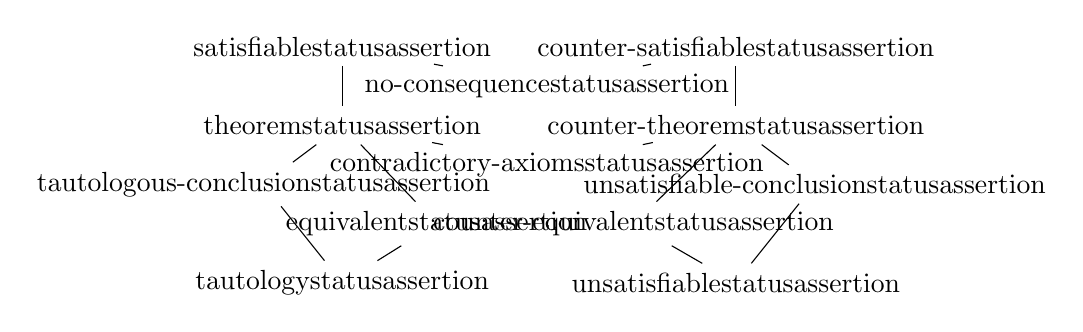
\begin{tikzpicture}
    \node (sat) at (1,4) {\attval{satisfiable}{status}{assertion}};
    \node (csat) at (6,4) {\attval{counter-satisfiable}{status}{assertion}};
    \node (thm) at (1,3) {\attval{theorem}{status}{assertion}};
    \node (cthm) at (6,3) {\attval{counter-theorem}{status}{assertion}};
    \node (tcon) at (0,2.25) {\attval{tautologous-conclusion}{status}{assertion}};
    \node (eqv) at (2.2,1.75) {\attval{equivalent}{status}{assertion}};
    \node (noc) at (3.6,3.5) {\attval{no-consequence}{status}{assertion}};
    \node (cax) at (3.6,2.5) {\attval{contradictory-axioms}{status}{assertion}};
    \node (ceqv) at (4.7,1.75) {\attval{counter-equivalent}{status}{assertion}};
    \node (ucon) at (7,2.25) {\attval{unsatisfiable-conclusion}{status}{assertion}};
    \node (taut) at (1,1) {\attval{tautology}{status}{assertion}};
    \node (usat) at (6,1) {\attval{unsatisfiable}{status}{assertion}};
    \draw (sat) -- (noc);
    \draw (sat) -- (thm);
    \draw (csat) -- (noc);
    \draw (csat) -- (cthm);
    \draw (thm) -- (tcon);
    \draw (thm) -- (cax);
    \draw (cthm) -- (cax);
    \draw (thm) -- (eqv);
    \draw (cthm) -- (ucon);
    \draw (cthm) -- (ceqv);
    \draw (tcon) -- (taut);
    \draw (eqv) -- (taut);
    \draw (ucon) -- (usat);
    \draw (ceqv) -- (usat);
  \end{tikzpicture}
\end{scriptsize}
\end{myfig}
\end{omgroup}

\begin{omgroup}[id=type-assertions]{Type Assertions}

In the last section, we have discussed the \element{type} elements in \element{symbol}
declarations. These were axiomatic (and thus {\indextoo{theory-constitutive}}) in
character, declaring a symbol to be of a certain type, which makes this information
available to type checkers that can check well-typedness (and thus plausibility) of the
represented mathematical objects.

\begin{omtext}
However, not all type information is axiomatic, it can also be deduced from other sources
knowledge. We use the same \element{type} element we have discussed in
{\sref{type-axioms}} for such \inlinedef{\defii{type}{assertions},
  i.e. non-constitutive statements that inform a type-checker}. In this case, the
\element{type} element can occur at top level, and even outside a \element{theory}
element (in which case they have to specify their home theory in the
\attribute{theory}{type} attribute).
\end{omtext}

{\Mylstref{term-declaration}} contains a type assertion $x+x\colon evens$, which makes the
information that doubling an integer number results in an even number available to the
reasoning process.

\begin{lstlisting}[label=lst:term-declaration,
  caption={A Term declaration in \omdoc.},
  index={type,assertion}]
<type xml:id="double-even.td" system="#POST" 
      theory="adv.int" for="plus" just-by="#double-even">
  <m:math>
    <m:apply><m:plus/>
      <m:ci type="integer">X</m:ci>
      <m:ci type="integer">X</m:ci>
    </m:apply>
  </m:math>
  <m:math>
    <m:csymbol definitionURL="http://cds.omdoc.org/integers/evens"/>
  </m:math>
</type>

<Assertion xml:id="double-even" type="lemma" theory="adv.int">
  <FMP>
    <m:math>
      <m:apply><m:forall/>
        <m:bvar><m:ci xml:id="x13" type="integer">X</m:ci></m:bvar>
        <m:apply><m:in/>
          <m:apply><m:plus/>
            <m:ci definitionURL="x13" type="integer">X</m:ci>
            <m:ci definitionURL="x13" type="integer">X</m:ci>
          </m:apply>
          <m:csymbol definitionURL="http://cds.omdoc.org/nat/evens"/>
        </m:apply>
      </m:apply>
    </m:math>
  </FMP>
</assertion>
\end{lstlisting}
The body of a type assertion contains two mathematical objects, first the type of
the object and the second one is the object that is asserted to have this
type.
\end{omgroup}

\begin{omgroup}[id=alternative]{Alternative Definitions}

  In contrast to what we have said about {\twintoo{conservative}{extension}s} at the end
  of {\sref{definitions}}, mathematical documents often contain multiple definitions for a
  concept or mathematical object. However, if they do, they also contain a careful
  analysis of equivalence among them. \omdoc allows us to model this by providing the
  \element{alternative} element.  Conceptually, an alternative definition or axiom is
  just a group of assertions that specify the equivalence of logical formulae. Of course,
  alternatives can only be added in a consistent way to a body of mathematical knowledge,
  if it is guaranteed that it is equivalent to the existing ones.  

\begin{definition}[id=alternative.def]
  The \attribute{for}{alternative} on the {\eldef{alternative }} points to the primary
  definition or assertion.  Therefore, \element{alternative} has the attributes
  \attribute{entails}{alternative} and \attribute{entailed-by}{alternative}, that
  specify {\element{assertion}s} that state the necessary entailments. It is an
  {\indextoo{integrity condition}} of \omdoc that any \element{alternative} element
  references at least one \element{definition} or \element{alternative} element that
  entails it and one that it is entailed by (more can be given for convenience). The
  \attribute{entails-thm}{alternative}, and \attribute{entailed-by-thm}{alternative}
  attributes specify the corresponding assertions. This way we can always reconstruct
  equivalence of all definitions for a given symbol. As alternative definitions are not
  theory-constitutive, they can appear outside a \element{theory} element as long as
  they have a \attribute{theory}{alternative} attribute.
\end{definition}
\end{omgroup}

\begin{omgroup}[short=Assertional Statements,id=assertional-statements]{Assertional Statements}

There is another distinction for statements that we will need in the following. Some kinds
of mathematical statements add information about the mathematical objects in question,
whereas other statements do not. For instance, a symbol declaration only declares an
unambiguous name for an object.
\begin{definition}[display=flow,id=assertional.def]
  We will call the following \omdoc elements
  \adefii{assertional}{assertional}{element}: \element{axiom} (it asserts central
  properties about an object), \element{type} (it asserts type properties about an
  object), \element{definition} (this asserts properties of a new object), and of course
  \element{assertion}.
\end{definition}

The following elements are considered non-assertional: \element{symbol} (only a name is
declared for an object), \element{alternative} (here the assertional content is carried
by the \element{assertion} elements referenced in the structure-carrying attributes of
\element{alternative}).  For the elements introduced below we will discuss whether they
are assertional or not in their context. In a nutshell, only statements introduced by the
module {\ADTmodule{spec}} (see {\sref{adt}}) will be assertional.
\end{omgroup}
\end{module}
\end{omgroup}

\begin{omgroup}[id=examples]{Mathematical Examples in OMDoc}
\begin{module}[id=examples]

In mathematical practice examples play a great role, e.g. in concept formation as
witnesses for definitions or as either supporting evidence, or as counter-examples for
conjectures.  Therefore examples are given status as primary objects in \omdoc.
Conceptually, we model an example $\cE$ as a pair $(\cW,\bA)$, where
$\cW=(\cW_1,\ldots,\cW_n)$ is an $n$-tuple of mathematical objects and $\bA$ is an
assertion. If $\cE$ is an example for a mathematical concept given as an \omdoc symbol
$\bS$, then $\bA$ must be of the form $\bS(\cW_1,\ldots,\cW_n)$.
  
If $\cE$ is an example for a conjecture $\bC$, then we have to consider the situation more
carefully. We assume that $\bC$ is of the form $\cQ\bD$ for some formula $\bD$, where
$\cQ$ is a sequence $\cQ_1W_1,\ldots,\cQ_mW_m$ of $m\geq n=\#\cW$ quantifications of using
quantifiers $\cQ_i$ like $\forall$ or $\exists$.  Now let $\cQ'$ be a sub-sequence of
$m-n$ quantifiers of $\cQ$ and $\bD'$ be $\bD$ only that all the $W_{i_j}$ such that the
$\cQ_{i_j}$ are absent from $\cQ'$ have been replaced by $\cW_j$ for $1\leq j\leq n$.  If
$\cE=(\cW,\bA)$ supports $\bC$, then $\bA=\cQ'\bD'$ and if $\cE$ is a counter-example for
$\bC$, then $\bA=\neg\cQ'\bD'$.
  
\begin{definition}[id=example.def]
  \omdoc specifies this intuition in an {\eldef{example}} element that contains
  mathematical vernacular as a \element[ns-elt=h]{p} elements for the description and
  $n$ mathematical objects (the witnesses). It has the attributes
\begin{description}
\item[\attribute{for}{example}] specifying for which concepts or assertions
    it is an example.  This is a reference to a {\indextoo{whitespace-separated
    list}} of {\indextoo{URI}} references to \element{symbol},
    \element{definition}, or \element{assertion} elements.
\item[\attribute{type}{example}] specifying the aspect, the value is one of
  \attval{for}{type}{example} or \attval{against}{type}{example}
\item[\attribute{assertion}{example}] a reference to the assertion $\bA$
  mentioned above that formally states that the witnesses really form an example for the
  concept of assertion. In many cases even the statement of this is non-trivial
  and may require a proof.
\end{description}
\end{definition}

\element{example} elements are considered
\twinalt{non-assertional}{assertional}{element} in \omdoc, since the assertional part is
carried by the \element{assertion} element referenced in the
\attribute{assertion}{example} attribute.

Note that the list of mathematical objects in an \element{example} element does not
represent multiple examples, but corresponds to the argument list of the symbol, they
exemplify. In the example below, the symbol for monoid is a three-place relation (see the
type declaration in {\mylstref{symbol}}), so we have three witnesses.

\begin{lstlisting}[label=lst:example,mathescape,
  caption={An \omdoc representation of a mathematical example},
  index={example,for,type,assertion}]
<symbol name="strings-over"/>
<definition xml:id="strings.def" for="strings-over">$\ldots$ $A^*$ $\ldots$</definition>
<symbol name="concat"/>
<definition xml:id="concat.def" for="concat">$\ldots$ $::$ $\ldots$</definition>
<symbol name="empty-string"/>
<definition xml:id="empty-string.def" for="empty-string">$\ldots$ $\epsilon$ $\ldots$</definition>
$\ldots$
<assertion xml:id="string.struct.monoid" type="lemma">
  <h:p>$(A^*,::,\epsilon)$ is a monoid.</h:p>
  <FMP>$mon(A^*,::,\epsilon)$</FMP>
</assertion>
$\ldots$
<example xml:id="mon.ex1" for="monoid" type="for"
        assertion="string.struct.monoid">
  <h:p>The set of strings with concatenation is a monoid.</h:p>
  <OMA id="nat-strings">
    <OMS cd="strings" name="strings"/>
    <OMS cd="setname1" name="N"/>
  </OMA>
  <OMS cd="strings" name="concat"/>
  <OMS cd="strings" name="empty-string"/>
</example>

<assertion xml:id="monoid.are.groups" type="false-conjecture">
 <h:p>Monoids are groups.</h:p>
 <FMP>$\allcdot{S,o,e}{mon(S,o,e)\rightarrow\excdot{i}{group(S,o,e,i)}}$</FMP>
</assertion>

<example xml:id="mon.ex2" for="#monoids.are.groups" type="against"
        assertion="strings.isnt.group">
  <h:p>The set of strings with concatenation is not a group.</h:p>
  <OMR href="#nat-strings"/>
  <OMS cd="strings" name="strings"/>
  <OMS cd="strings" name="concat"/>
  <OMS cd="strings" name="empty-string"/>
</example>

<assertion xml:id="strings.isnt.group" type="theorem">
  <h:p>$(A^*,::,\epsilon)$ is a monoid, but there is no inverse function for it.</h:p>
</assertion>
\end{lstlisting}

In {\mylstref{example}} we show an example of the usage of an \element{example} element
in \omdoc: We declare constructor symbols {\snippet{strings-over}}, that takes an
{\indextoo{alphabet}} $A$ as an argument and returns the set $A^*$ of
{\indextoo{strings}s} over $A$, {\snippet{concat}} for {\twintoo{strings}{concatenation}}
(which we will denote by $::$), and {\snippet{empty-string}} for the
{\twintoo{empty}{string}} $\epsilon$.  Then we state that $\cW=(A^*,::,\epsilon)$ is a
monoid in an \element{assertion} with {\snippet{xml:id="string.struct.monoid"}}.  The
\element{example} element with {\snippet{xml:id="mon.ex1"}} in {\mylstref{example}} is
an example for the concept of a monoid, since it encodes the pair $(\cW,\bA)$ where $\bA$
is given by reference to the assertion {\snippet{string.struct.monoid}} in the
\attribute{assertion}{example} attribute.  Example {\snippet{mon.ex2}} uses the pair
$(\cW,\bA')$ as a {\indextoo{counter-example}} to the {\twintoo{false}{conjecture}}
{\snippet{monoids.are.groups}} using the assertion {\snippet{strings.isnt.group}} for
$\bA'$.
\end{module}
\end{omgroup}

\begin{omgroup}[id=inline-statements]{Inline Statements}
\begin{module}[id=inline-statements]
 
Note that the infrastructure for statements introduced so far does its best to mark up the
interplay of formal and informal elements in mathematical documents, and make explicit the
influence of the context and their contribution to it. However, not all statements in
mathematical documents can be adequately captured directly.  Consider for instance the
following situation, which we might find in a typical mathematical textbook.
\begin{sblockquote}
  {\presbf{Theorem 3.12}}: {\presem{In a monoid $M$ the left unit and the right unit
      coincide, we call it the {\presbf{unit}} of $M$.}}
\end{sblockquote}
The overt role of this text fragment is that of a mathematical theorem --- as indicated by
the cue word ``{\presbf{Theorem}}'', therefore we would be tempted represent it as an
\element{omtext} element with the value \attval{theorem}{type}{attribute} for the
\attribute{type}{attribute} attribute. But the relative clause is clearly a
{\indextoo{definition}} (the {\indextoo{definiens}} is even marked in boldface). What we
have here is an aggregated verbalization of two mathematical statements. In a simple case
like this one, we could represent this as follows:

\begin{lstlisting}[mathescape,caption=A Simple-Minded Representation of {\presbf{Theorem 3.12}}]
<assertion type="theorem" style="display=flow">
  <h:p>In a monoid $M$, the left unit and the right unit coincide,</h:p>
</assertion>
<definition for="unit" style="display:flow">
   <h:p>we call it the <term role="definiendum" name="unit">unit</term> of $M$</h:p>
</definition>
\end{lstlisting}

But this representation remains unsatisfactory: the definition is not part of the theorem,
which would really make a difference if the theorem continued after the inline
definition. The real problem is that the inline definition is linguistically a
phrase-level construct, while the \element{omtext} element is a discourse-level
construct. However, as a phrase-level construct, the inline definition cannot really be
taken as stand-alone, but only makes sense in the context it is presented in (which is the
beauty of it; the re-use of context). With the \element[ns-elt=h]{span} element and its
\attribute[ns-elt=h]{verbalizes}{span}, we can do the following:

\begin{lstlisting}[mathescape,caption=An Inline Definition]
<assertion xml:id='unit-unique' type="theorem" >
  <h:p>In a monoid M, the left unit and the right unit coincide,
    <h:span verbalizes="#unit-def">we call it the unit of M</h:span>.</h:p>
</assertion>
<symbol name="unit"/>
<definition xml:id="unit-def" for="unit" just-by='#unit-unique'>
  <h:p>We call the (unique) element of a monoid M that acts as a left 
    and right unit the <term role="definiendum" name="unit">unit</term> of M.</h:p>
</definition>
\end{lstlisting}

thus we would have the phrase-level markup in the proper place, and we would have an
explicit version of the definition which is standalone\footnote{Purists could use the CSS
  attribute \attribute{style}{definition} on the \element{definition} element with
  value {\attvalshort{display:none}{style}} to hides it from the document; it might also
  be placed into another document altogether}, and we would have the explicit relation
that states that the inline definition is an ``abbreviation'' of the standalone
definition.\ednote{we probably also need inline examples and inline assertions, see
  \tracticket{1498}.}
\end{module}
\end{omgroup}

\begin{omgroup}[id=theories-contexts]{Theories as Structured Contexts}
\begin{module}[id=theories]
\omdoc provides an infrastructure for mathematical theories as first-class objects that
can be used to structure larger bodies of mathematics by functional aspects, to serve as a
framework for semantically referencing mathematical objects, and to make parts of
mathematical developments reusable in multiple contexts. The module {\STmodule{spec}}
presented in this chapter introduces a part of this infrastructure, which can already
address the first two concerns. For the latter, we need the machinery for complex theories
introduced in {\sref{complex-theories}}.

\begin{definition}[id=theory.def]
  Theories are specified by the {\eldef{theory}} element in \omdoc, which has a required
  \attribute[ns-attr=xml]{id}{theory} attribute for referencing the theory. Furthermore,
  the \element{theory} element can have the \attribute[ns-elt=om]{cdbase}{theory}
  attribute that allows to specify the \attribute{cdbase}{OMS} this theory uses for
  disambiguation on \element[ns-elt=om]{OMS} elements (see {\sref{openmath}} for a
  discussion).
\end{definition}
Additional information about the theory like a title or a short description can be given
in the \element{metadata} element. AfTer this, any {\indextoo{top-level}} \omdoc
element can occur, including the theory-constitutive elements introduced in
{\srefs{statements-constitutive}{definitions}}, even \element{theory} elements
themselves. Note that theory-constitutive elements may {\emph{only}} occur in
\element{theory} elements.

\begin{definition}[id=tgroup.def]
  Theories can be structured like documents e.g. into sections and the like (see
  {\sref{sectioning}} for a discussion) via the {\eldef{tgroup}} element, which behaves
  exactly like the \element{omdoc} element introduced in {\sref{sectioning}} except that
  it also allows theory-constitutive elements, but does not allow a
  \attribute{theory}{omdoc} attribute, since this information is already given by the
  dominating \element{theory} element.\footnote{This element has been introduced to keep
    \omdoc validation manageable: We cannot directly use the \element{omdoc}
    element,since there is no simple, context-free way to determine whether an
    \element{omdoc} is dominated by a \element{theory} element.}
\end{definition}  

\begin{presonly}
\begin{myfig}{simple-thy}{Theories in \omdoc}
\begin{scriptsize}
\begin{tabular}{|>{\tt}l|>{\tt}l|>{\tt}p{5.4truecm}|c|>{\tt}p{2truecm}|}\hline
{\rm Element}& \multicolumn{2}{l|}{Attributes\hspace*{2.25cm}} & M & Content  \\\hline
             & {\rm Req.}  & {\rm Optional}                    & D &           \\\hline\hline
 theory      &             & xml:id, class, style, cdbase, 
                             cdversion, cdrevision, cdstatus, cdurl, 
                             cdreviewdate                      & + & (\llquote{top+thc} | imports)*\\\hline
 imports     & from        & id, type, class, style            & + & \\\hline
 tgroup      &   & xml:id, modules, type, class, style         & +  & (\llquote{top+thc})* \\\hline
 \multicolumn{5}{|p{11cm}|}{where \llquote{top+thc} stands for top-level and
   theory-constitutive elements}\\\hline
\end{tabular}
\end{scriptsize}
\end{myfig}
\end{presonly}

\begin{omgroup}[id=inheritance]{Simple Inheritance}

\element{theory} elements can contain \element{imports} elements (mixed in
with the top-level ones) to specify inheritance: The main idea behind structured theories
and specification is that not all theory-constitutive elements need to be explicitly
stated in a theory; they can be inherited from other theories. Formally, the set of
theory-constitutive elements in a theory is the union of those that are explicitly
specified and those that are imported from other theories. This has consequences later on,
for instance, these are available for use in proofs. See
{\sref{proofs.justifications}} for details on availability of assertional statements in
proofs and justifications.

\begin{definition}[id=imports.def]
  The meaning of the {\eldef{imports}} element is determined by two attributes:
\begin{description}
\item[\attribute{from}{imports}] The value of this attribute is a
  {\twintoo{URI}{reference}} that specifies the \defii{source}{theory},
    i.e. the theory we import from.  The current theory (the one specified in
    the parent of the \element{imports} element, we will call it the
    \defii{target}{theory}) inherits the constitutive elements from the source
  theory.
\item[\attribute{type}{imports}] This optional attribute can have the values
  \attval{global}{type}{imports} and \attval{local}{type}{imports} (the former is
  assumed, if the attribute is absent): We call constitutive elements \defi{local} to
  the current theory, if they are explicitly defined as children, and else
  \defi{inherited}.  A \defii{local}{import} (an \element{imports} element with
  {\snippet{type="local"}}) only imports the local elements of the source theory, a
  {\indextoo{global}} import also the inherited ones.
\end{description}
\end{definition}

The meaning of nested \element{theory} elements is given in terms of an implicit imports
relation: The inner theory imports from the outer one. Thus
\begin{lstlisting}[label=lst:nested-thy,index={theory}]
<theory xml:id="a.thy">
  <symbol name="aa"/>
  <theory xml:id="b.thy">
    <symbol name="cc"/>
    <definition xml:id="cc.def" for="cc" type="simple">
       <OMS cd="a.thy" name="af"/>
    </definition>
  </theory>
</theory>
\end{lstlisting}
is equivalent to 
\begin{lstlisting}[label=lst:nested-thy-equiv,index={theory}]
<theory xml:id="a.thy"><symbol name="aa"/></theory>
<theory xml:id="b.thy">
  <imports from="#a.thy" type="global"/>
  <symbol name="cc"/>
  <definition xml:id="cc.def" for="cc" type="simple">
     <OMS cd="a.thy" name="af"/>
  </definition>
</theory>
\end{lstlisting}
In particular, the symbol {\snippet{cc}} is visible only in theory {\snippet{b.thy}}, not
in the rest of theory {\snippet{a.thy}} in the first representation.

Note that the inherited elements of the current theory can themselves be inherited in the
source theory. For instance, in the {\mylstref{def-group}} the {\snippet{left-inv}} is the
only local axiom of the theory {\snippetin{group}}, which has the inherited axioms
{\snippet{closed}}, {\snippet{assoc}}, {\snippet{left-unit}}.

In order for this import mechanism to work properly, the
{\twintoo{inheritance}{relation}}, i.e.  the relation on theories induced by the
\element{imports} elements, must be {\indextoo{acyclic}}. There is another, more subtle
constraint on the inheritance relation concerning multiple inheritance.  Consider the
situation in {\mylstref{multiple-inheritance}}: here theories {\snippet{A}} and
{\snippet{B}} import theories with {\snippet{xml:id="mythy"}}, but from different
URIs. Thus we have no guarantee that the theories are identical, and semantic integrity of
the theory {\snippet{C}} is at risk. Note that this situation might in fact be totally
unproblematic, e.g. if both URIs point to the same document, or if the referenced
documents are identical or equivalent. But we cannot guarantee this by content markup
alone, we have to forbid it to be safe.

\begin{lstlisting}[label=lst:multiple-inheritance,
  caption={Problematic Multiple Inheritance},
  index={theory,symbol,axiom,imports}]
<theory xml:id="A">
  <imports from="http://red.com/theories.omdoc#mythy"/>
</theory>
<theory xml:id="B">
  <imports from="http://blue.org/cd/all.omdoc#mythy"/>
</theory>
<theory xml:id="C"><imports from="#A"/><imports from="#B"/></theory>
\end{lstlisting}

Let us now formulate the constraint carefully, 
\begin{definition}[display=flow,id=base.uri.def]
  the \defii{base}{URI} of an {\xml} document is the {\indextoo{URI}} that has been
  used to retrieve it.
\end{definition}
We adapt this to \omdoc theory elements: the base URI of an imported theory is the URI
declared in the \attribute{cdbase}{theory} attribute of the \element{theory} element
(if present) or the base URI of the document which contains it\footnote{Note that the base
  URI of the document is sufficient, since a valid \omdoc document cannot contain more
  than one \element{theory} element for a given
  \attribute[ns-attr=xml]{id}{theory}}. For theories that are imported along a chain of
global imports, which include {\twintoo{relative}{URI}s}, we need to employ
{\twintoo{URI}{normalization}} to compute the {\twintoo{effective}{URI}}.  Now the
constraint is that any two imported theories that have the same value of the
\attribute[ns-attr=xml]{id}{theory} attribute must have the same base URI. Note that
this does not imply a global unicity constraint for \attribute[ns-attr=xml]{id}{theory}
values of \element{theory} elements, it only means that the mapping of theory
identifiers to URIs is unambiguous in the dependency cone of a theory.

In {\mylstref{def-group}} we have specified three algebraic theories that gradually build
up a theory of groups importing theory-constitutive statements (symbols, axioms, and
definitions) from earlier theories and adding their own content. The theory
{\snippetin{semigroup}} provides symbols for an operation {\snippetin{op}} on a base set
{\snippetin{set}} and has the axioms for closure and associativity of
{\snippetin{op}}. The theory of monoids imports these without modification and uses them
to state the {\snippet{left-unit}} axiom. The theory {\snippetin{monoid}} then proceeds to
add a symbol {\snippetin{neut}} and an axiom that states that it acts as a left unit with
respect to {\snippetin{set}} and {\snippetin{op}}.  The theory {\snippetin{group}}
continues this process by adding a symbol {\snippetin{inv}} for the function that gives
inverses and an axiom that states its meaning.

\begin{lstlisting}[label=lst:def-group,escapechar=\%,mathescape,
  caption={A Structured Development of Algebraic Theories in \omdoc},
  index={theory,symbol,axiom,imports}]
<theory xml:id="semigroup">
  <symbol name="set"/><symbol name="op"/>
  <axiom xml:id="closed"> $\ldots$ </axiom><axiom xml:id="assoc"> $\ldots$ </axiom>
</theory>

<theory xml:id="monoid">
  <imports from="#semigroup"/>
  <symbol name="neut"/><symbol name="setstar"/>
  <axiom xml:id="left-unit">
    <h:p>%\tt{neut}% is a left unit for %\tt{op}%.</h:p><FMP>$\allcdot{x\in{\tt{set}}}{{\tt{op}}(x,{\tt{neut}})=x}$</FMP>
  </axiom>
  <definition xml:id="setstar.def" for="setstar" type="implicit">
    <h:p>$\cdot^*$ subtracts the unit from a set </h:p><FMP>$\allcdot{S}{S^*=S\backslash\set{\tt{unit}}}$</FMP>
  </definition>
</theory>

<theory xml:id="group"> 
  <imports from="#monoid"/>
  <symbol name="inv"/>
  <axiom xml:id="left-inv">
    <h:p>For every $X\in\tt{set}$ there is an inverse ${\tt{inv}}(X)$ wrt. %\tt{op}%.</h:p>
  </axiom>
</theory>
\end{lstlisting}

The example in {\mylstref{def-group}} shows that with the notion of theory inheritance it
is possible to re-use parts of theories and add structure to specifications. For instance
it would be very simple to define a theory of {\twintoo{Abelian}{semigroup}s} by adding a
{\twintoo{commutativity}{axiom}}.

\begin{omtext}
  The set of symbols, axioms, and definitions available for use in proofs in the importing
  theory consists of the ones directly specified as \element{symbol}, \element{axiom},
  and \element{definition} elements in the target theory itself (\inlinedef{we speak of
    \defi{local} axioms and definitions in this case} and the ones that are inherited from
  the source theories via \element{imports} elements.  Note that these symbols, axioms,
  and definitions (\inlinedef{we call them \defi{inherited}}) can consist of the local
  ones in the source theories and the ones that are inherited there.
\end{omtext}

The local and inherited symbols, definitions, and axioms are the only ones
available to mathematical statements and proofs. If a symbol is not available in
the home theory (the one given by the dominating \element{theory} element or the
one specified in the \attribute{theory}{statement} attribute of the statement),
then it cannot be used since its semantics is not defined.
\end{omgroup}

\begin{omgroup}[id=identifying]{OMDoc Theories as Content Dictionaries}
\begin{oldpart}{The discussion here depends on the upcoming OM3 standard and MathML3
    recommendation. The material is provisional on the expected outcome and may change in
    the future.}


\begin{omtext}
  In {\sref{mobj}}, we have introduced the {\openmath} and {\cmathml} representations for
  mathematical objects and formulae. One of the central concepts there was the notion that
  the representation of a symbol includes a pointer to a document that defines its
  meaning.  In the {\openmath} standard, these documents are identified as
  \atwinalt{{\openmath} content dictionaries}{OpenMath}{content}{dictionary}, the
  {\mathml} recommendation is not specific.  In the examples above, we have seen that
  \omdoc documents can contain definitions of mathematical concepts and symbols, thus
  they are also candidates for ``defining documents'' for symbols.  By the {\openmath}2
  standard~\cite{BusCapCar:2oms04} suitable classes of \omdoc documents can act as
  {\openmath} content dictionaries (\inlinedef{we call them \omdoc \adefii{content
      dictionaries}{content dictionary}{OMDoc}}; see {\sref{sub-languages.cd}}).  The main
  distinguishing feature of \omdoc content dictionaries is that they include
  \element{theory} elements with {\twintoo{symbol}{declaration}s} (see
  {\sref{definitions}}) that act as the targets for the pointers in the symbol
  representations in {\openmath} and {\cmathml}. The theory name specified in the
  \attribute[ns-attr=xml]{id}{theory} attribute of the \element{theory} element takes
  the place of the {\snippet{CDname}} defined in the \atwinalt{{\openmath} content
    dictionary}{OpenMath}{content}{dictionary}.
\end{omtext}

Furthermore, the {\indextoo{URI}} specified in the \attribute{cdbase}{theory} attribute
is the one used for disambiguation on \element[ns-elt=om]{OMS} elements (see
{\sref{openmath}} for a discussion).
  
For instance the symbol declaration in {\mylstref{symbol}} can be referenced as\ednote{is
  this really the right {\texttt{cdbase?}}}
\begin{lstlisting}
<OMS cd="elAlg" name="monoid" cdbase="http://omdoc.org/algebra.omdoc"/>
\end{lstlisting}
if it occurs in a theory for elementary algebra whose
\attribute[ns-attr=xml]{id}{theory} attribute has the value {\snippet{elAlg}} and which
occurs in a resource with the URI \url{http://omdoc.org/algebra.omdoc} or if the
\attribute{cdbase}{theory} attribute of the \element{theory} element has the value
\url{http://omdoc.org/algebra.omdoc}.

To be able to act as an {\openmath}2 {\twintoo{content dictionary}{format}}, \omdoc must
be able to express {\twintoo{content dictionary}{metadata}} (see {\mylstref{omcd}} for an
example). For this, the \element{theory} element carries some optional attributes that
allow to specify the administrative metadata of {\openmath} content dictionaries.

\begin{omtext}
  The \attribute{cdstatus}{theory} attribute specifies \inlinedef{the {\defii{content
        dictionary}{status}}}, which can take one of the following values:
  \attval{official}{cdstatus}{theory} (i.e. approved by the {\openmath} Society),
  \attval{experimental}{cdstatus}{theory} (i.e. under development and thus liable to
  change), \attval{private}{cdstatus}{theory} (i.e. used by a private group of
  {\openmath} users) or \attval{obsolete}{cdstatus}{theory} (i.e. only for archival
  purposes). The attributes \attribute{cdversion}{theory} and
  \attribute{cdrevision}{theory} jointly specify \inlinedef{the \defii{content
      dictionary}{version number}, which consists of two parts, a major \defi{version} and
    a \defi{revision}, both of which are non-negative integers}. For details between the
  relation between content dictionary status and versions consult the {\openmath}
  standard~\cite{BusCapCar:2oms04}.
\end{omtext}

\begin{omtext}
Furthermore, the \element{theory} element can have the following attributes:
\begin{description}
\item[\attribute{cdbase}{theory}] for the {\twintoo{content dictionary}{base}} which, when
  combined with the content dictionary name, forms a unique identifier for the content
  dictionary. It may or may not refer to an actual location from which it can be
  retrieved.
\item[\attribute{cdurl}{theory}] for a valid URL where the source file for the content
  dictionary encoding can be found.
\item[\attribute{cdreviewdate}{theory}] for \inlinedef{the \defii{review}{date} of the
    content dictionary, i.e. the date until which the content dictionary is guaranteed to
    remain unchanged}.
\end{description}
\end{omtext}
\end{oldpart}
\end{omgroup}
\end{module}
\end{omgroup}

\begin{omgroup}[id=st.strict]{Strict Translations}

  We will now give the a formal\ednote{do we really want to call it ``formal''?} semantics
  of the {\STmodule{spec}} elements in terms of strict \omdoc (see
  {\sref{strict}}).\ednote{what do we do if there is both FMP and CMPs in an
    axiom?}\ednote{what do we do if there is more than one symbol per
    definition?}\ednote{what do we do for non-simple definitions}

\begin{center}\lstset{frame=none,numbers=none,lineskip=-.7ex,aboveskip=-.5em,belowskip=-1em}
  \begin{tabular}{|p{6cm}|p{6cm}|}\hline
    pragmatic & strict\\\hline
{
\begin{lstlisting}[numbers=none,frame=none,mathescape]
<axiom name="$\llquote{n}$" xml:id="$\llquote{i}$">
  $\llquote{body}$
</axiom>
\end{lstlisting}
}&{
\begin{lstlisting}[numbers=none,frame=none,mathescape]
<object name="$\llquote{n}$" xml:id="$\llquote{i}$">
  $\llquote{body}$
</object>
\end{lstlisting}
}\\\hline{
\begin{lstlisting}[numbers=none,frame=none,mathescape]
<symbol name="$\llquote{n}$">
  <type system="$\llquote{s}$">$\llquote{t}$</type>
</symbol>
<definition type="simple"
            xml:id="$\llquote{i}$" for="$\llquote{n}$">
  $\llquote{body}$
</definition>
\end{lstlisting}
}&{
\begin{lstlisting}[numbers=none,frame=none,mathescape]
<object name="$\llquote{n}$" xml:id="$\llquote{i}$">
  <type system="$\llquote{s}$">$\llquote{t}$</type>
  <definition>$\llquote{body}$</definition>
</object>
\end{lstlisting}
}\\\hline 
\end{tabular}
\end{center}
\end{omgroup}
\end{omgroup}

%%% Local Variables: 
%%% mode: latex
%%% TeX-master: "main"
%%% End: 

% LocalWords:  lang adt lst mathescape en monoide mon qtconst def cd dc cmp om
% LocalWords:  nat eq xref int suc requation exp rec ref qttheory sst dec csat
% LocalWords:  isnt peano ness bvar mtext concat empystrg setname OMR xlink Ai
% LocalWords:  href Luehts MMiSS qaulified mythy Bi CiA CiB escapechar setstar
% LocalWords:  gim mobj CDname elAlg es td adv ci csymbol definitionURL aa cc
% LocalWords:  equiv cdbase openmath ns elt attr cdversion FMP pres af
% LocalWords:  cdrevision cdstatus cdurl cdreviewdate OMBIND OMATTR multi bool
% LocalWords:  metadata arities OMA sgrp forall thm mW inv Req wrt omcd
% LocalWords:  nmueller ple Inline omtext cthm tcon eqv noc cax ceqv ucon usat
% LocalWords:  tgroup omdoc thc
